\documentclass[11pt]{article}
\usepackage[utf8]{inputenc}
\usepackage{booktabs}
\usepackage{multicol}
\usepackage{amsmath}
\usepackage{amsfonts}
\usepackage{fullpage}
\usepackage{amsmath,amssymb,amsthm}
\usepackage{tikz,lipsum,lmodern}
\usepackage[most]{tcolorbox}
\usepackage{graphicx}
\def\R{{\mathbb{R}}}
\def\N{{\mathbb{N}}}
\def\Z{{\mathbb{Z}}}


\begin{center}
    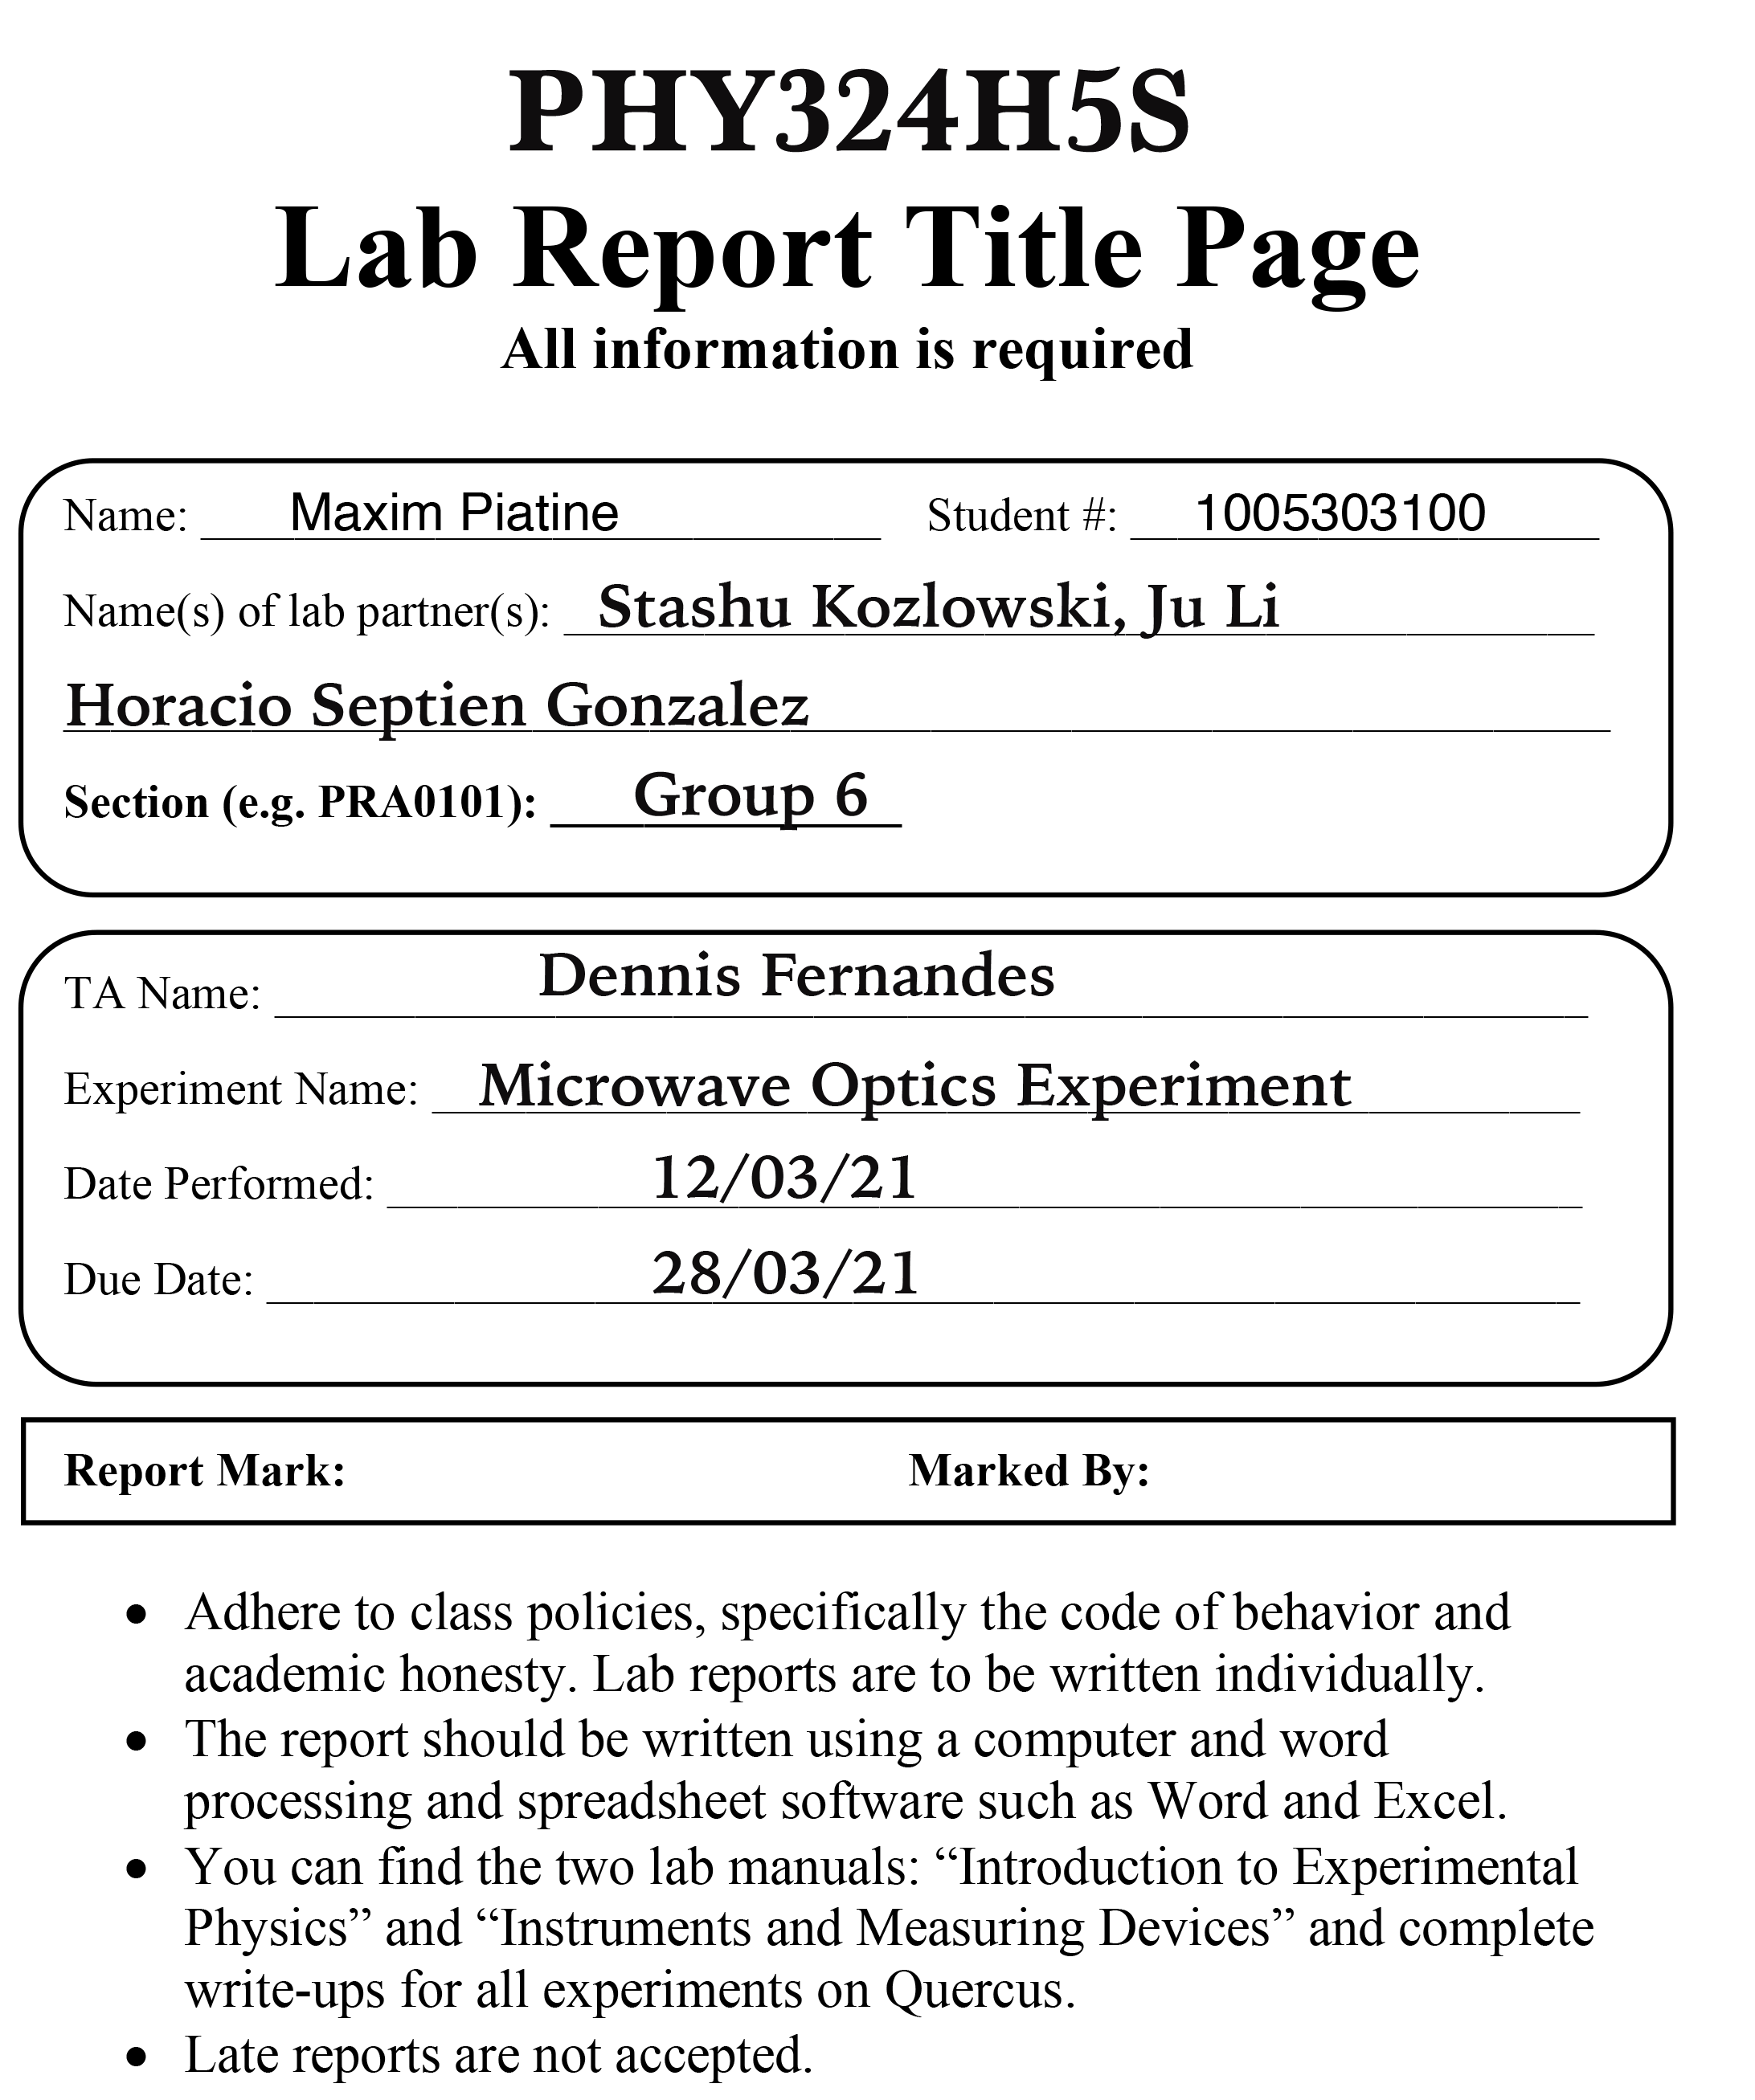
\includegraphics[width=17cm]{MicrowaveOptics.png}
\end{center}

\newpage
\begin{document}
\section*{Abstract}
In this laboratory, the purpose was to investigate the polarization, how a polarizer is affected depending on the transmitter's rotation, reader, and filter—moreover, a deeper understanding of the double-slit interference and the intensity of waves depending on the angles.\\
Firstly, Malus' law breaks down a fundamental theory of transverse waves when interacting with the various transmissions or receptions according to their respective degrees. When the receiver is being rotated on its axis, the receiving current will follow a cosine function path. As well as the transmitter when it is being rotated on its axis. Proving the fundamental law of Malus' law, no matter what degree the receiver or transmitter will be rotated on, it would follow the oscillatory cosine function. Furthermore, if a slit comes into contact between the receiver and reader, then the current strength would be greater than when there is no filter separating both horns. That is due to the depolarized waves not being able to slide through the slits to affect the field's intensity. However, when the slit is rotated, the maximum signal strength came from the slit being at $45^\circ$ and not when the slit was inline with the vertically polarized microwave. That goes against the theory; but, it could be due to human error or that the microwave's components were in line with the reader.\\
Finally, the double-slit interference followed the theoretical pattern. The maximas and minimas were perfectly aligned to be in the theoretical angles. However, theoretically, with the wavelength at $2.85cm$, there are infinite amounts of maximas and minimas when $n$ approaches infinity due to its double-slit interference nature. Nonetheless, experimental angles are within the theoretical angles at specific $n$'s. They are deducting that the experimental results follow the theoretical ones. \\
Overall, the experiment was a success with minor uncertainties.

\section*{Introduction}
The purpose of this laboratory activity is to investigate various applications of microwave optics such as the phenomenon of polarization and how a polarizer can be used to alter the polarization of a microwave radiation, and the double-slit interference which provides an insight on the intensity of waves beyond the aperture depending on the angle of detection.\\
Polarization is a transverse wave that has a specific geometrical orientation when it comes to the oscillations. Comparing to the different types of oscillations, such as linear, circular, and elliptical polarization. The microwave radiation coming from the transmitter in this experiment is linearly polarized along the transmitter diode axis. Since the transmitter is vertically aligned then the waves would be vertically polarized. 
\begin{center}
    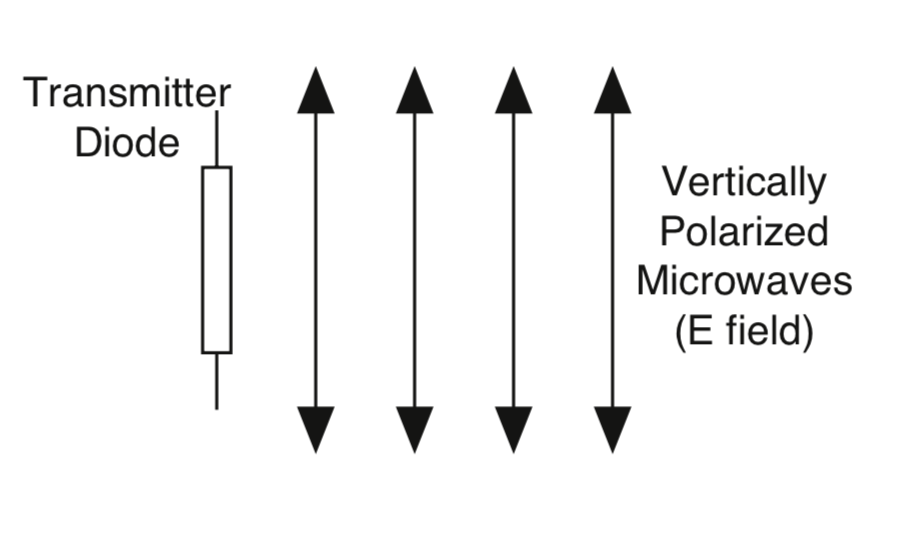
\includegraphics[width=7cm]{figure1.png}\\\textbf{Figure 1}: The microwave radiation from the transmitter is linearly polarized along the transmitter diode. As the radiation propagates through space, the electric field remains aligned with the axis of the diode. 
\end{center}
If the transmitter diode would be at an angle $\theta$ then it would detect the component of the incident electric field that was aligned along its axis.
\begin{center}
    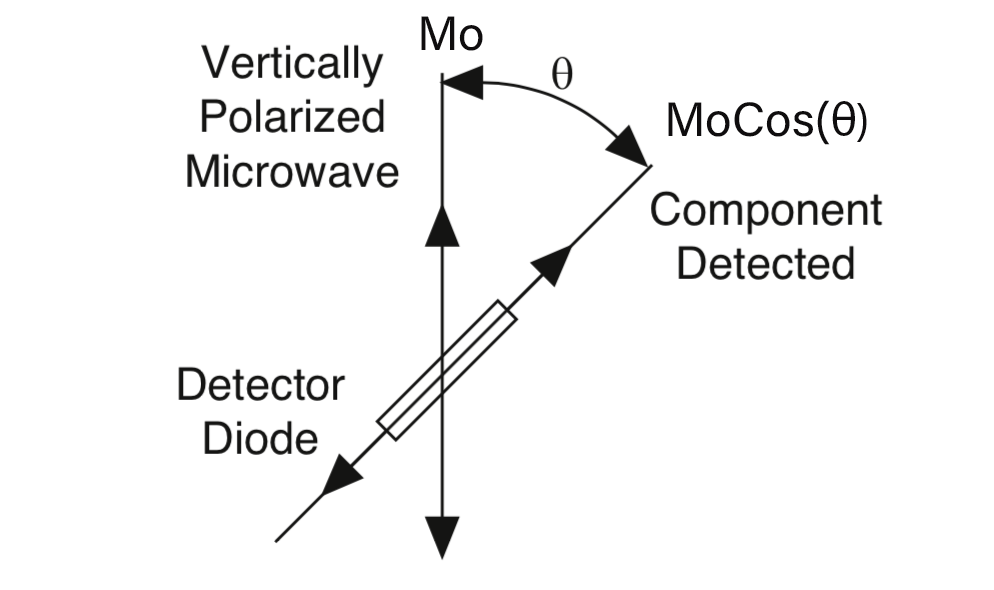
\includegraphics[width=7cm]{figure2 copy.png}\\\textbf{Figure 2}: The effect of the electric field depending on the angle $\theta$ as a component towards the vertically polarized microwave.
\end{center}
If the receiver meter reading $M$ is proportional to the electric field component $E$ along its axis, the meter would read the relationship:
\begin{equation}
    M=M_o\cos\theta
\end{equation}
 from Figure 2, $M_o$ is the initial receiver meter when the angle $\theta$ is at zero; meaning, when detector is inline with the vertically polarized microwave.\\
The intensity of a linearly polarized electromagnetic wave is directly proportional to the square of the electric field $I=kE^2$. The receiver's meter reading is directly proportional to the incident microwave's intensity, then the meter would read a relationship of:
\begin{equation}
    M=M_o\cos^2\theta
\end{equation}
Theoretically, following Malus' law.\\
The double-slit interference determines the intensity of the wave beyond the aperture depending on the angle $\theta$ of detection. The wave diffracts into two waves which superpose in the space beyond the apertures. Similar to the standing wave pattern, there are points in space where maxima are formed and others where minima are formed. For two thin slits separated by a distance $d$, maxima will be found at angles such that: 
\begin{equation}
    d\sin\theta=n\lambda
\end{equation}
Where $\theta$ is the angle of detection, $\lambda$ is the wavelength of the incident radiation, and $n \in \Z$. Moreover, minima will be found at angles such that: 
\begin{equation}
    d\sin\theta=\frac{n\lambda}{2}
\end{equation}
\begin{center}
    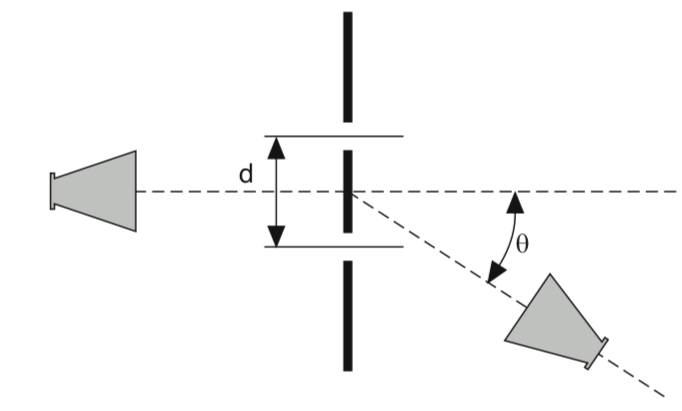
\includegraphics[width=7cm]{figure 3.png}\\\textbf{Figure 3}: The transmitter is placed at an angle $\theta$ and the waves are travelling through the slits separated with $d$ distance.
\end{center}

\section*{Procedure}
Follow procedure from "Experiment 5: Polarization" and "Experiment 6: Double-Slit Interference" in the "Microwave Optics" Lab Manual.

\begin{center}
    Experiment 5: Polarization
\end{center}
Arrange the equipment as shown in Figure 5.3 (refer to Lab Manual) and adjust the Receiver controls for nearly full-scale meter deflection.\\

\noindent Loosen the hand screw on the back of the Receiver and rotate the Receiver in increments of ten degrees. At each rotational position, record the meter reading.\\

\noindent There is no point on rotating the receiver beyond $180\circ$ degrees because theoretically it follows a cosine function. Meaning, the meter reading will oscillate with a period of $\pi$ or $180^\circ$.\\

\noindent Set up the equipment as shown in Figure 5.4 (in Lab Manual). Reset the Receivers angle to $0^\circ$ degrees (the horns should be oriented as shown with the longer side horizontal).\\

\noindent Record the meter reading when the Polarizer is aligned at 0, 22.5, 45, 67.5 and 90-degrees with respect to the horizontal.\\

\noindent Remove the Polarizer slits. Rotate the Receiver so the
axis of its horn is at right angles to that of the Transmitter. Record the meter reading. Then replace the Polarizer slits and record the meter readings with the Polarizer slits horizontal, vertical, and at $45^\circ$ degrees.

\begin{center}
    Experiment 6: Double-Slit Interference
\end{center}
Arrange the equipment as shown in Figure 6.2 (Refer to Lab Manual for Figures). Use the Slit Extender Arm, two Reflectors, and the Narrow Slit Spacer to construct the double slit. (We recommend a slit width of about 1.5 cm.) Be precise with the alignment of the slit and make the setup as symmetrical as possible.\\

\noindent Adjust the Transmitter and Receiver for vertical polarization (0°) and adjust the Receiver controls to give a full-scale reading at the lowest possible amplification.\\

\noindent Rotate the rotatable Goniometer arm (on which the Receiver rests) slowly about its axis. Observe the meter readings.\\

\noindent Reset the Goniometer arm so the Receiver directly faces the Transmitter. Adjust the Receiver controls to obtain a meter reading of 1.0. Now set the angle $\theta$ to each of the values shown in Table 6.1 (Refer to Lab Manual for Figures). At each setting record the meter reading in the table. (In places where the meter reading changes significantly between angle settings, you may find it useful to investigate the signal level at intermediate angles.)\\

\noindent Keep the slit widths the same, but change the distance between the slits by using the Wide Slit Spacer instead of the Narrow Slit Spacer. Because the Wide Slit Space is $50\%$ wider than the Narrow Slit Spacer (90mm vs 60mm) move the Transmitter back $50\%$ so that the microwave radiation at the slits will have the same relative intensity. Repeat the measurements.
(You may want to try other slit spacings as well.)\\

\section*{Data and Analysis}
The purpose of this experiment is to investigate the polarization, how a polarizer can affect the polarization of microwave radiation. It also investigates the double-slit interference that provides insight into the intensity of waves beyond the aperture, depending on the detection angle.\\
When analyzing the electric field's effect depending on the angle $\theta$ as a component, the reading meter collects information on the field's strength based on the angle the detector diode is from the polarized microwave. From figure 2, in theory, the reading meter follows a formula depending on the angle; theoretically, the formula follows equation (1). 
\newpage
\begin{center}
    \textbf{Graph 1}: Meter Reading from Angle Component \\
    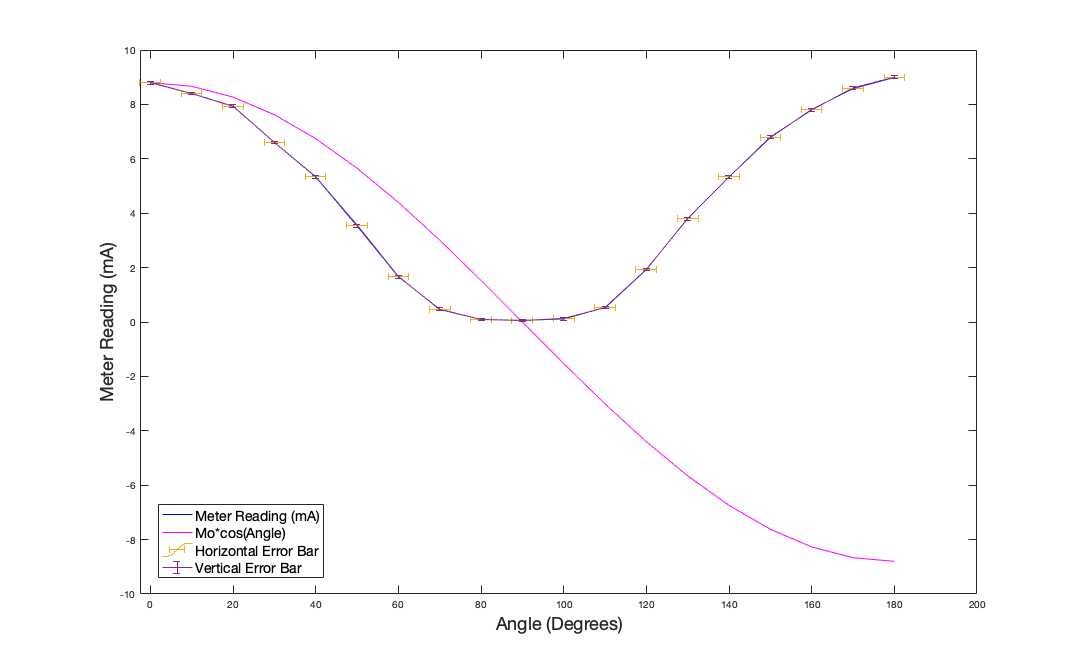
\includegraphics[width=17cm]{q.png}\\\textbf{Graph 1}: From the theoretical computations of MatLab, the pink graph was created via code. The pink graph follows a cosine function that takes in the angle difference between the vertically polarized microwave and the transmitter diode. Furthermore, at $\theta=0$ the input $M_o$ is $8.8 mA$. The blue graph overshadowed by the purple and yellow graph is the data collected from the experiment. The independent value $x$ is the angle in degrees, the dependent value $y$ is the meter reading per each angle measured in milliampere. The horizontal error bars have a $\pm 2.5^\circ$ and the vertical error bars have a $\pm 0.05 mA$.
\end{center}
The relationship between the acquired data and the theoretical, there is a pattern around the experimental data to look like an oscillatory function since if the procedure stated to go above and beyond $180^\circ$ then it would have repeated itself due to its nature.  The theoretical cosine graph in equation (1) seems to correspond to the experimental; if the experimental data had an opposing current.\\
Therefore, Malus' law states equation (2), which theoretically corresponds to the experimental fitted function. Since Malus' equation considers the cosine function to be squared, then graphically, the plot will never be negative since the range of cos would be between 0 and 1. The incident wave, being the wave that approaches the reader, is at $\theta=0$ is $8.8mA$.\\
\newpage
\begin{center}
    \textbf{Graph 2}: Theoretical Current Readings Against Experimental\\
    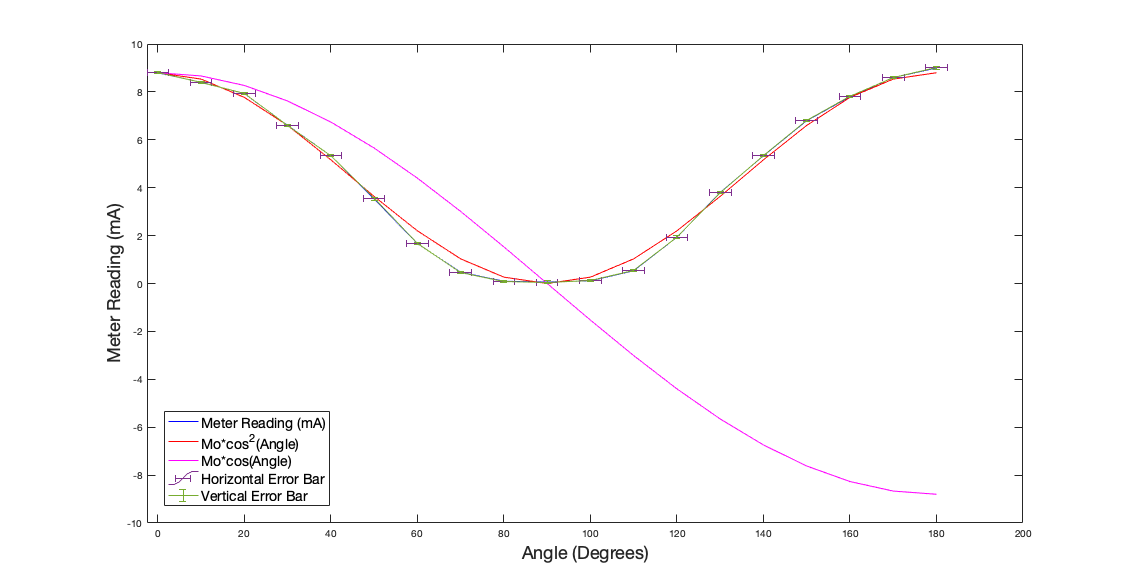
\includegraphics[width=17cm]{w.png}\\\textbf{Graph 2}: The independent value $x$ of the graph is the angle measured in degrees, and the dependent value $y$ is the meter reading measured in milliampere. From the data collected the blue graph was created. That blue graph is overshadowed by the horizontal error bar of $\pm 2.5^\circ$ and vertical error bar of $\pm 0.05 mA$ in purple and green respectively. The red graph is a representation of equation (2) $M_o\cos^2\theta$ and the pink graph is a representation of equation (1) $M_o\cos\theta$. 
\end{center}
When adding rotating the polarizer the reader will receive various field strengths due to the waves' transverse nature.  Based on the graph presented in the appendix, when the polarizer is at $0^\circ$, the field's strength is at its peak. Compared to the polarizer being at $90^\circ$, the field strength is nearly zero; due to the polarizer being completely perpendicular to the polarizing slit. According to Malus' law (equation(2)), the theoretical calculations add up to the experimental process. There is a trend between the angle of the polarizer and the strength of the microwaves that the detector is receiving. Moreover, due to the increasing angle, the meter reading gradually gets weaker. Therefore, the incident microwave decreases depending on the angle of the polarizer. Based on the calculations done in the appendix, per each degree, the polarizer shifts the field's strength decreases by $-0.1 \pm 0.01mA$. Nevertheless, the graph seems to be a repetition from the reader being rotated, since the concept is the same just opposite horns are being rotated, confirming Malus' law. \\
If the polarizer slit is being rotated by maintaining the polarizer vertically correct, then at $45^\circ$, the current was the strongest than when the slit was aligned or perpendicular to the polarizer. Theoretically, it does not match equation (2), considering that if the polarizer is vertically oriented, then the slit at $90^\circ$ would be the maximum. However, that could be due to the wave components parallel to the receiver being introduced and not blocked off.\\
On the other hand, when removing the polarizing slit, the recorded reading slit was measured at $0.06 mA$, nearly the same as it was blocked off. The signal is more robust when there is a polarizing filter compared to when there is none because of the concentration waves going through the slit. Moreover, if adding another slit, the signal would be more substantial due to the polarizing slit cleaning up the signal and removing the depolarizing microwaves.\\

\\Setting the slits at a certain distance will make a double-slit interference that will provide an oscillatory pattern. Therefore, determining the maximum and minimum points is based on equation (3) and equation (4).  When determining the angle of maximums and minimums, the transmitter needs to be placed at a certain angle, as shown in figure 3. 
\begin{center}
    \textbf{Graph 3}: Minima $\&$ Maxima of Wide Double-Slit Interference\\
    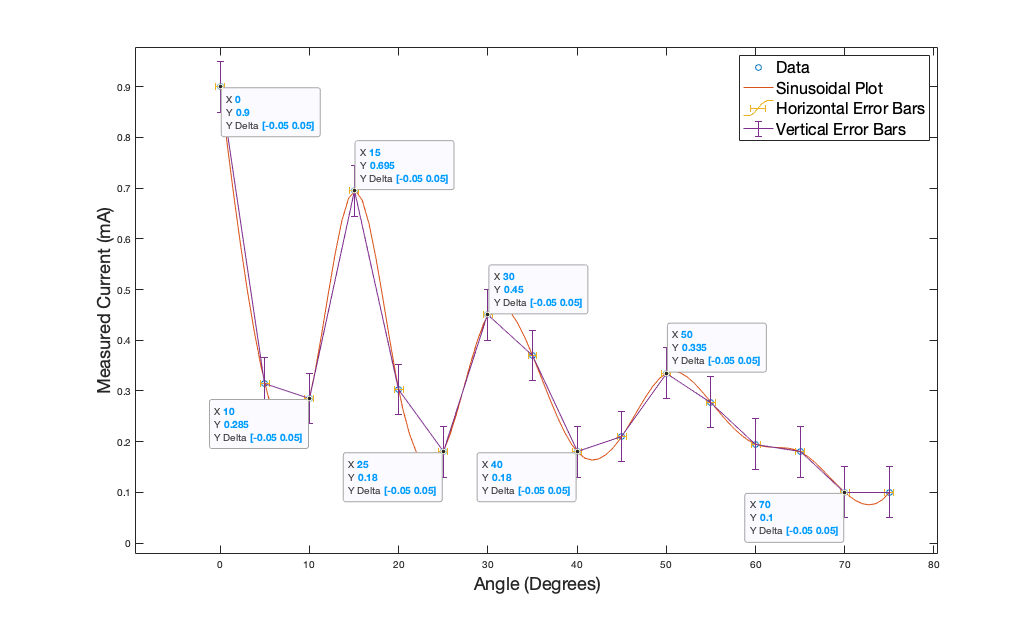
\includegraphics[width=18cm]{Ex6.png}\\\textbf{Graph 3}: From the collected raw data and the wide slits, this graph was able to be created with the help of MatLab. The independent value $x$ is the angle measured in degrees, the dependent value $y$ is the measured current measured in milliampere. The maximum and minimums are identified using Data Tip function in MatLab. The sinusoidal plot in red follows the data points, to identify the maximum and minimum points. The yellow horizontal bars are due to the uncertainties in the measured degrees being $\pm 0.5^\circ$. The purple vertical error bars are due to the uncertainty in the measured current being $\pm 0.05 mA$. 
\end{center}
The graph presented seems to follow double-slit interference graph patterns. Each dip can be represented with a natural number $n$. Moreover, each dip is considered as the minimas, and each small peak can be considered the maximas. Therefore, for each angle increase, the minima and maxima decrease gradually, precisely like a theoretical double-slit interference, which means, if the maximum and minimum angles were to be compared to equations of diffraction (equation (1) and (2))— knowing the wavelength $\lambda$ of $2.85cm$ and the distance between the wide slits of $1.5$. Then the angles should line up.\\
However, after calculating all the theoretical maximum and minimum angles, there seems to have vast amounts of maximum angles theoretically than found in the graph. The same applies to the minimal theoretical values calculated. Many minimal and maximal angles mean that the interference patterns have many more dips that can be accounted for $n$ the integer depending on the number of dips. Comparing to graph 3, the number of oscillations would be increased by 10. Nevertheless, the theoretical angles of maximas and minimas corresponded to the experimental maximas and minimas found on the graph. Furthermore, the experimental uncertainties lie within the theoretical values (Appendix Table 1).\\
The diffraction pattern seems to drop in intensity when $n$ naturally approaches infinity. Due to the concentration of waves hitting the center and $n$ approaching infinity, the waves' concentration diminishes. In other words, the microwave travels the least distance to the center with the most significant amount of constructive interference. Further away, there would be less constructive interference, explaining why the intensity is dropped as $n$ approaches infinity. If it were a single slit pattern, then there would not be such a high concentration of maximas and minimas than the double-slit pattern. 


\section*{Discussion and Conclusion}
To conclude, the purpose of this experiment was to investigate various applications of microwave optics such as polarization and how polarizing slits can be used to alter the polarization of microwave radiation and the double-slit interference, which provides an insight into the intensity of waves beyond the aperture depending on the angle of detection. \\
To test the polarization, one of the procedures is to maneuver the meter reading to an appropriate degree to register the microwaves. The reader followed a function squared from equation (2) since the meter does not register a negative current thrown at it. Nevertheless, the reader provided insight into the microwaves' oscillation depending on the receiver, which confirms Malus' law. On the other hand, making the reader still while the polarizing waves were being rotated would not change the rotating the reader's outcome due to Malus' law following a cosine squared function. Therefore, confirming the theory of the graphical analysis.\\ 
Theoretically, if the polarizing slit were in line with the microwaves, the reader would receive the most current according to Malus' law. However, at $45^\circ$, the current was at its maximum according to the receiver. That goes against the theory, but it could have been due to the waves' components being parallel to the receiver—possibly human error when aligning the polarizing slit at a specific angle. Nonetheless, what is know is that when the polarizing slit was vertical and horizontal, the current was near zero. Moreover, when removing the polarizing slit, the current was less potent than when the slit has blocked the microwaves. That can be explained via microwaves' concentration being projected through the polarizing slits removing the depolarizing microwaves. \\

\\Lastly, for double-slit interference, the theoretical angles to which would have a maximum or minimum intensity would follow equation (3) and equation (4) respectively. Considering the theoretical interference with the wavelength of $2.85cm$ would hold a lot of maximums and minimums if $n$ approaches infinity. Nonetheless, the experimental maximum and minimum angles obtained from graph 3 lay within the theoretical values. Therefore, making the experimental in line with the theoretical. 

\newpage
\section*{Appendix}
Wagih, Ghobriel: Lab manual I: Introduction to Experimental Physics.
\begin{center}
    \textbf{Appendix 1}: Polarizer's Affect on the Incident Microwave\\
    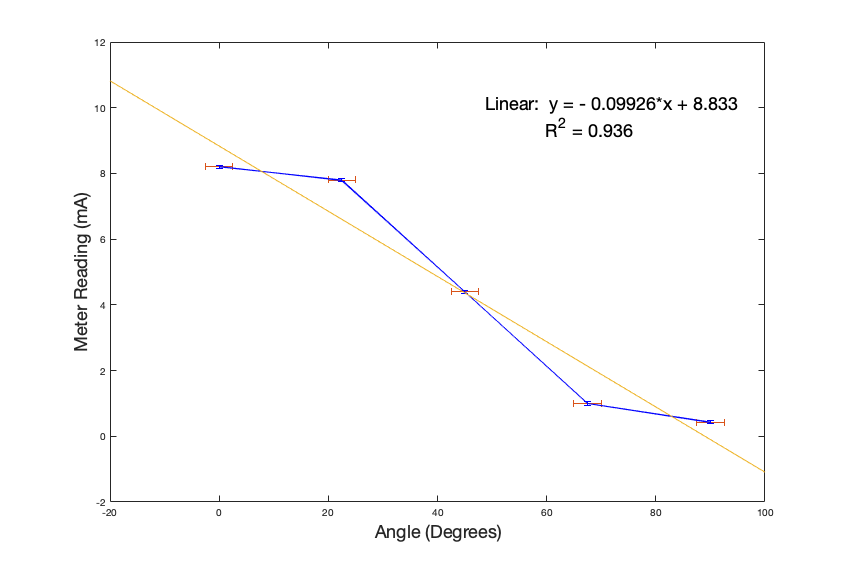
\includegraphics[width=15cm]{ex5.4.png}\\\textbf{Appendix 1}: The independent value $x$ of the graph is the angle measured in degrees, and the dependent value $y$ is the meter reading measured in milliampere. From the data collected the blue graph was created. The horizontal error bar is $\pm 2.5^\circ$ and vertical error bar is $\pm 0.05 mA$. The slope of the linear trend graph is $-0.09926 \pm 0.014986658 \frac{mA}{Degree}$. Moreover, the $R^2$ value of the graph is $0.936$ indicates that the data is $93.6\%$ of the variation in the $y$ data is due to the variation in the $x$ data; giving a perfect slope of the alignment of the data.
\end{center}
Excel Linear Regression: $0.01498mA$
\begin{center}
 \caption{\textbf{Table 1}: Wide slits Experimental $\&$ Theoretical Angles of Double-Slit Interference} 
 \begin{tabular}{||c c c c||} 
 \hline
 Max Exp Angle & Min Exp Angle & Theo Max Angles & Theo Min Angles\\ [0.5ex] 
 \hline\hline
 $15\pm0.5$ & $10\pm0.5$ & 15.2 & 10.45\\ 
 \hline
 $30\pm0.5$ & $25\pm0.5$ & 30.4 & 25.65\\
 \hline
 $50\pm0.5$ & $40\pm0.5$ & 49.4 & 39.9\\
 \hline
 - & $72.5\pm0.5$ & - & 72.1\\ [1ex] 
 \hline
\end{tabular}
\\\textbf{Table 1}: The experimental values seem to lay within the theoretical values because of the uncertainties. The two left most columns were found via experimental analysis within graphs. The two rightmost columns were found via calculations to compare with the theoretical. 
\end{center}
Theoretical Maximum Angles Calculations:
\[d\sin\theta=n\lambda \Rightarrow \theta = \sin^{-1}(\frac{n\lambda}{d})\]
\[\theta=\sin^{-1}(\frac{(1)(2.85cm)}{1.5cm})=1.9\]
Theoretical Minimum Angles Calculations:
\[d\sin\theta=\frac{n\lambda}{2} \Rightarrow \theta = \sin^{-1}(\frac{n\lambda}{2d})\]
\[\theta=\sin^{-1}(\frac{(1)(2.85cm)}{(2)1.5cm})=0.95\]
\newpage
\begin{center}
    MatLab Codes:\\
    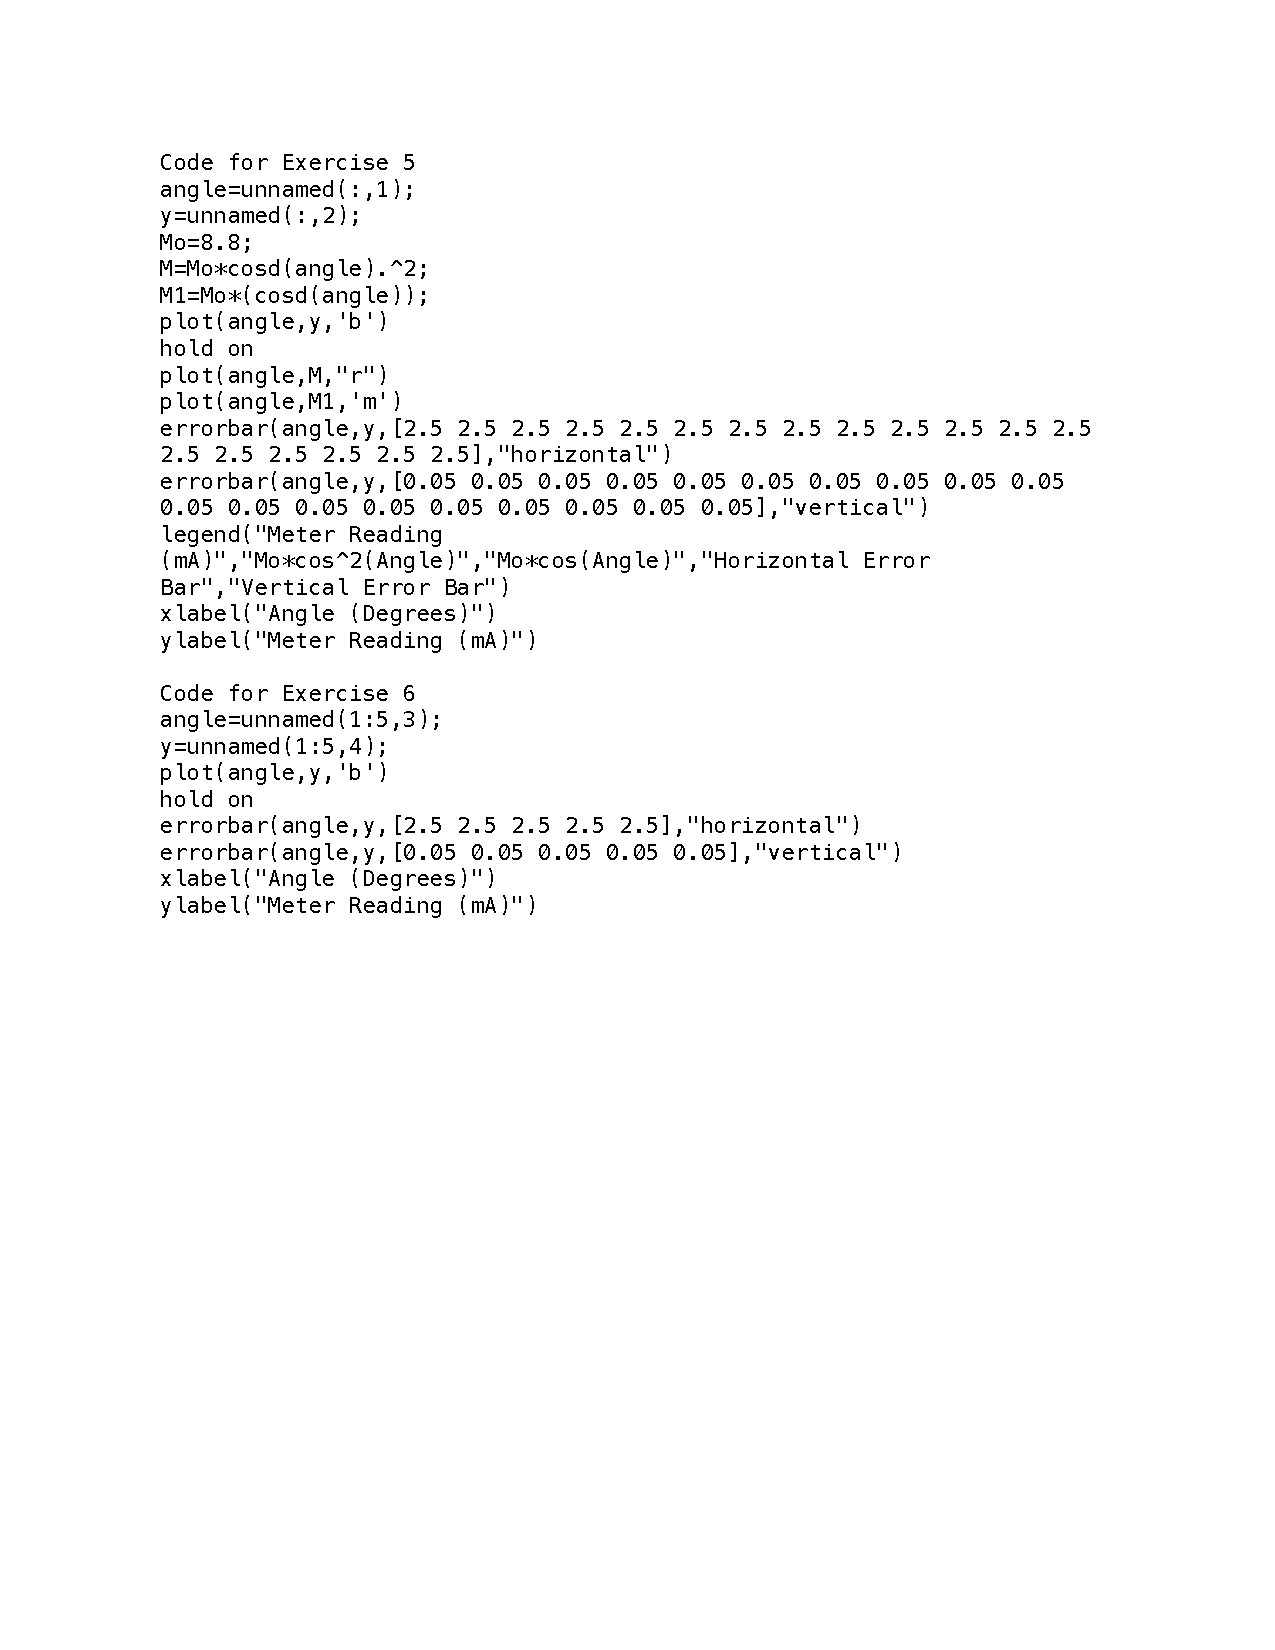
\includegraphics[width=16cm]{text.pdf}
\end{center}

\end{document}